\documentclass[12pt]{article}

\usepackage[left=2.5cm,top=2.5cm,right=2.5cm,bottom=2.5cm]{geometry}

%% Macros and packages go here

\usepackage{enumitem}
\usepackage[style=ieee, backend=biber]{biblatex}
\usepackage{hyperref}
\usepackage{minted}

\usepackage{graphicx}

\addbibresource{references.bib}

\begin{document}
\title{COMP0005 Algorithms: Group Coursework Report}
\author{Group Number: 54}
\date{Academic year 2025/26}
\maketitle
\vspace{-4em}
\section{Experimental framework overview}

\subsection{Framework design and architecture}
The framework empirically measures the asymptotic relationship between (search / insertion) operation times and the number of nodes in a balanced tree.
The $TestDataGenerator$ class contains four generators, namely random (uniform and normal) and ordered (ascending and descending), to suitably stress test insertions and searches for 2-3, LLRB and AVL trees.
Uniform sampling leads to best-case performance, as the keys are naturally self-balancing (the expected height of a vanilla BST is $O(logn)$ \cite{algorithms}).
Normal represents the average case; by the Central Limit Theorem, sampled data often take a normal distribution.
Ordered keys cause worst case behavior - maximal re-balances occur due to always inserting on one side of the tree.
The time to compare keys is controlled: every key has a constant string length $k$, so the cost of key comparisons is $O(1)$ with respect to the number of nodes, $n$, in the tree.
Due to lazy evaluation, the time cost of comparisons of fixed-length strings can vary, but for small $k$, as we chose, the difference is negligible.
This keeps the theoretical time complexity of searches and insertions for all trees to $O(logn)$.
The keys are generated numerically and cast into strings. To maintain numerical order when compared lexicographically as strings, decimals are truncated (by casting to a Python $int$), cast to $str$, and left-padded with 0's.
A string length ($k$ above) of 7 was chosen, giving $10^7$ unique keys.
Data are collected using the $ExperimentalFramework$ class.
The testing algorithm grows $m$ trees up to size $n$ and measures operation cost at intervals spaced by a geometric progression ratio $r=e^{ln(n)/data \ points}$ to spread the data points equally when plotting a log-graph.
$m$ = 250 ensures noise caused by processes such as context switching and garbage collection can be averaged away.
Measurements are taken for 250 data points across a wide range, $[1, n]$ where $n$ = $10^4$.
At each interval, an insertion is measured along with a search for a key inside and outside the tree.
 The $StatisticsFramework$ class processes the data for each experiment after it is collected.
It takes $log$ values at each interval, removes outliers (extreme values > 5 inter-quartile ranges above the upper quartile) and calculates: the PMCC, a quantitative measurement of linearity, to verify the relation; the RMSE, to give insight into the stability / predictability of a data structure's performance; mean values, standard deviations and standard errors for error bars; regression coefficients used to reason about the hidden constants in a data structure's implementation; and lastly, residuals, which help to interpret the mechanics of the trees (explored in section 2.1). The graphs are processed using Matplotlib.

\subsection{Hardware/software setup for experiments}
Hardware - Laptop: Apple MacBook Pro M4 (10 core CPU, 10 core GPU); Memory: 16GB LPDDR5X; 120 Gb$s^{-1}$ bandwidth \cite{wikiM4}; Cache: L1: 192 (instruction) + 128 KiB (data) per P core; 128 + 64 KiB per E core; L2: 16 MiB for P core cluster; 4 MiB for E core cluster.
Software - OS: MacOS Tahoe 26.3.1; Python Interpreter: 3.11.0; Python Libraries: timeit, random, matplotlib.
\vspace{-1em}

\section{Performance results}

\vspace{-2em}
\begin{figure}[htbp]
    \centering
    \begin{minipage}{0.48\textwidth}
        \centering
        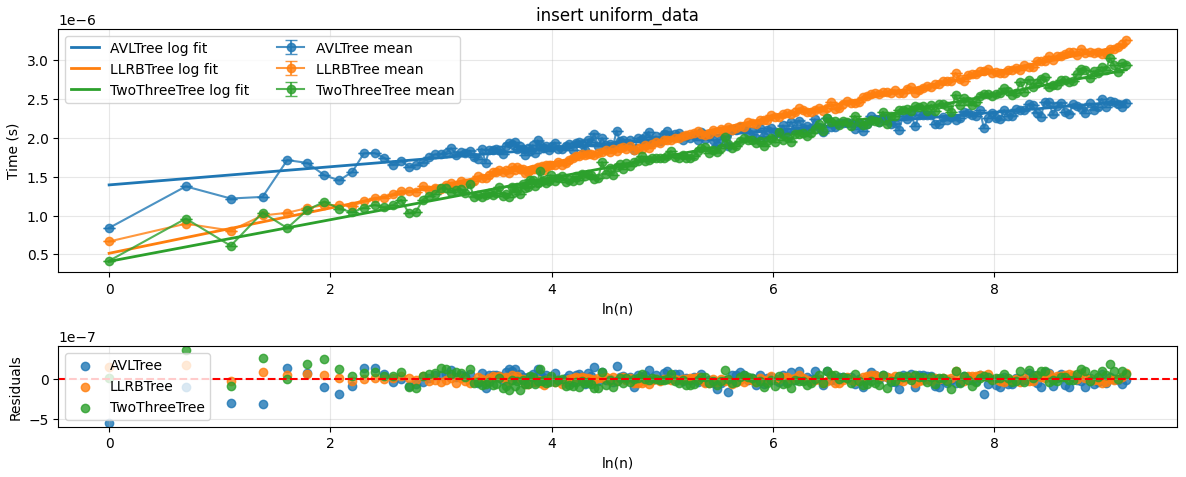
\includegraphics[width=\textwidth]{1.png}
        \vspace{-2em}
        \caption{Comparison of insertion time under uniformly distributed keys.}
        \label{fig:1}
    \end{minipage}
    \hfill
    \begin{minipage}{0.48\textwidth}
        \centering
        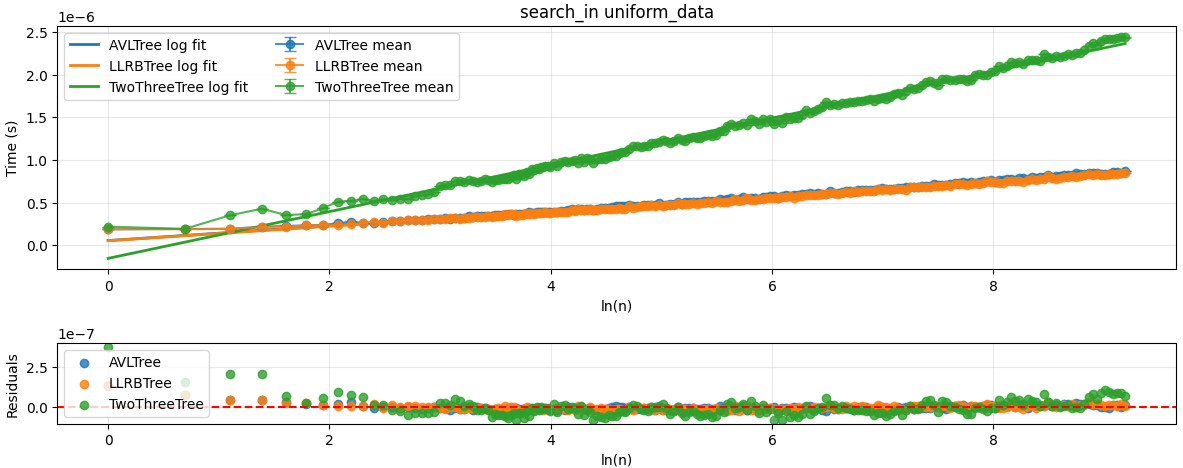
\includegraphics[width=\textwidth]{2.png}
        \vspace{-2em}
        \caption{Comparison of successful search time under uniformly distributed keys.}
        \label{fig:3}
    \end{minipage}
\end{figure}
\vspace{-2em}
\subsection{2-3 Tree}
With random input, the 2-3 tree gave low average insertion times - the gradients of the regression line for insertions are approximately $2.68\times 10^{-7}$s and $2.44 \times 10^{-7}$s under uniform and normal input respectively - this can be interpreted as the extra time cost in increasing the number of nodes by a factor of $e$. Insertions trigger local split operations when a node becomes overfull which rarely propagate far up the tree, making them inexpensive.

The experiments showed the main weakness of the 2-3 tree is searching. Across the four input-generation methods, the fitted slopes of successful-search had gradients ranging from about $2.69 \times 10^{-7}$s to $3.34 \times 10^{-7}$s, and unsuccessful-search gradients from about $2.60 \times 10^{-7}$s to $3.12 \times 10^{-7}$s. These values are about three times larger than the corresponding AVL and LLRB slopes. 

The plots in Figure 3 showed a step-like structure, especially for sorted and reverse-sorted data. Long horizontal segments correspond to periods where the tree height remains unchanged; steps appear when a new layer is created. The oscillating residuals suggest that even at the same height, performance strongly depends on the distribution of 2- and (more expensive to traverse) 3- nodes in the tree.
Ordered inputs revealed a second weakness: erratic insertion times. The scatter about the regression line was very high and the strength of the logarithmic fit deteriorated, with $R^2$ - a measure of how much variance the regression model captures - falling to about $0.50$ for sorted input and $0.43$ for reverse-sorted input. 
The spikes in the insertion graphs indicate the occurrence of cascading split operations through several layers of the tree. With sorted input, the cost of an insertion is determined by the number of 3-nodes above the rightmost leaf. If 2-nodes are viewed as binary 0s and 3-nodes as binary 1s, then sorted insertions behave like incrementing a binary counter, with binary carries causing split operations. So, expensive insertions occur at regular intervals, doubling in separation with every extra split. This explains the layered spike pattern observed in the sorted-input graph.
Overall, the 2-3 tree performs well when  average insertion throughput matters, but its search overhead and irregular insertion spikes make its runtime unpredictable, particularly when operating with worst-case data.

\begin{figure}[htbp]
    \centering
    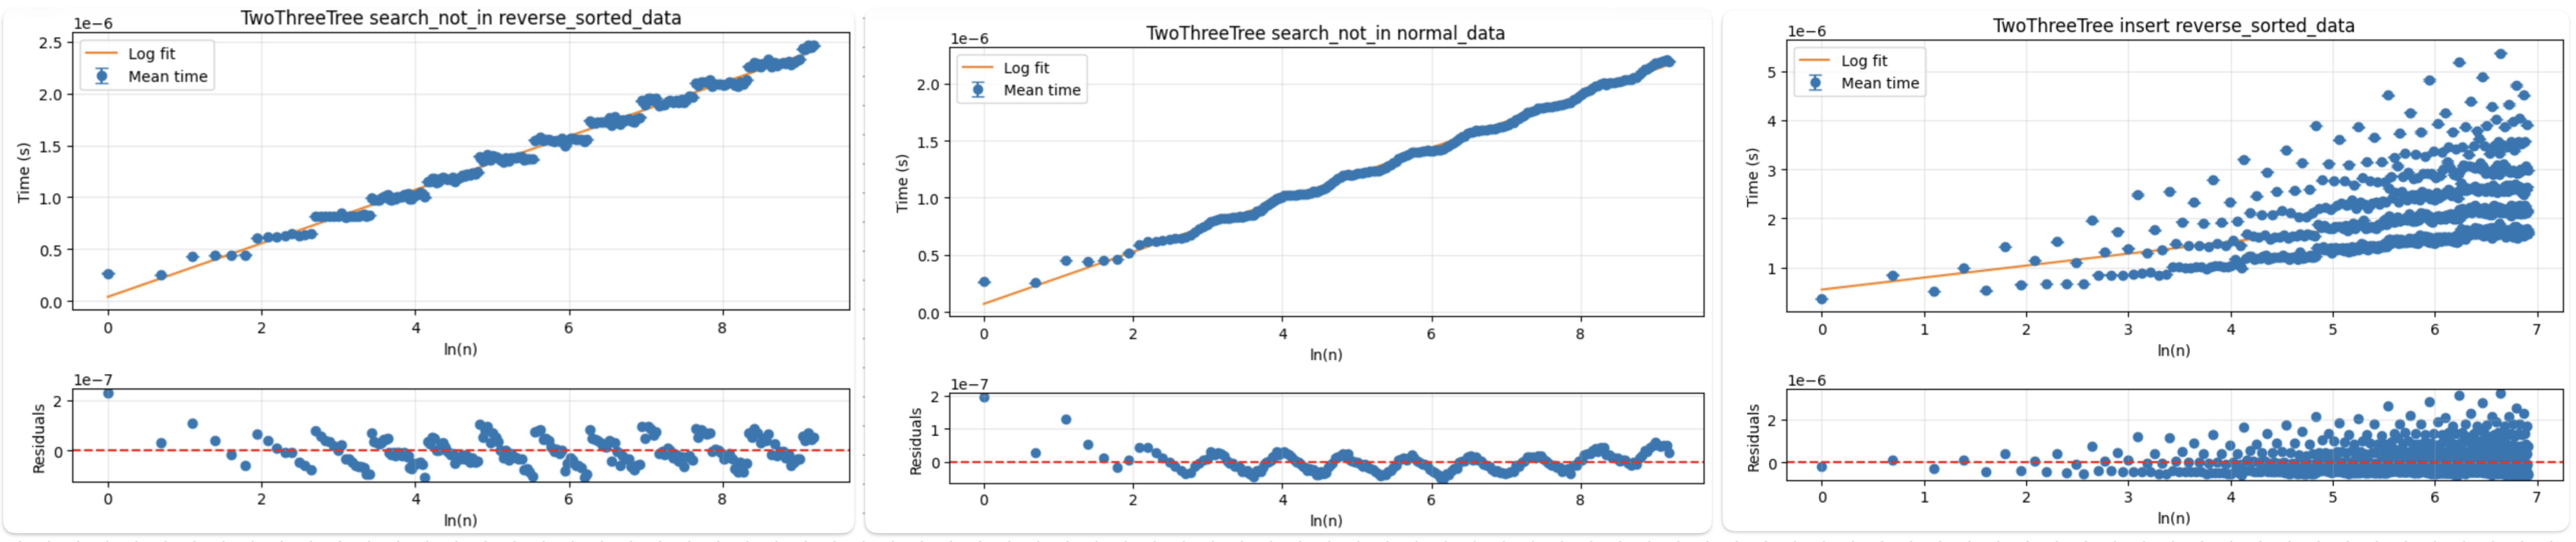
\includegraphics[width=0.96\textwidth]{4.png}
    \vspace{-1em}
    \caption{Representative 2-3 tree plots with residual patterns.}
\end{figure}
\vspace{-2em}
\subsection{LLRB Tree}
The LLRB tree performed strongly. For uniform and normal inputs, the insertion gradients are about $2.90 \times 10^{-7}$s and  $2.96 \times 10^{-7}$s, which are slower than the AVL tree, but still competitive. The search performance was also good. For successful searches, the fitted slopes are between $8.50 \times 10^{-8}$s and $9.57 \times 10^{-8}$s, and for unsuccessful searches between $7.03 \times 10^{-8}$s and $1.02 \times 10^{-7}$s.

This performance is consistent with the structure of LLRB tree. The LLRB tree implements 2-3 tree behavior with a BST representation, using cheap local rotations and colour flips for balancing.

The limitation of the LLRB tree appears under reverse-ordered insertion. The graph's fitted slope rises to about $3.62 \times 10^{-7}$ and $R^2$ drops to about $0.79$, showing that although the trend remains logarithmic, the sequence of rotations and colour flips becomes more irregular when the inserted elements come with biased order. Overall, the LLRB tree offers the best compromise between strong search performance and predictable insertion performance. 

The LLRB was not hindered by inserting sorted data. The left-leaning invariant explains this asymmetry. Sorted keys are inserted as right children, which are immediately rotated to the left, without causing colour flips, whereas reverse-sorted keys are inserted as left children, and can cause cascading operations upwards.

\vspace{-1em}
\subsection{AVL Tree}

The AVL tree is the fastest of the three implementations on average insertion time across all four input distributions.
Under uniform and normal inputs, the fitted insertion gradients are about $1.17 \times 10^{-7}$s and $1.14 \times 10^{-7}$s, which are the lowest between three implementations. Under the sorted and reverse-sorted inputs, AVL tree's insertion gradients are about $1.46 \times 10^{-7}$s and $1.27 \times 10^{-7}$s. This is significantly below the corresponding LLRB tree's and 2-3 tree's gradients. 

This performance is consistent with the implementation of AVL tree. The implementation now propagates a boolean flag up the recursion, stops checking ancestors once a subtree height no longer changes, and terminates further upward fix-up after a rotation restores local balance.

However, the speed comes with a clear cost in predictability. The insertion fit now captures only about $91\%$ of the variance under uniform and normal input, and only about $24\%$ under sorted and reverse-sorted input.

Search in the AVL tree is consistently efficient and predictable. The successful search gradients range from about $8.55 \times 10^{-8}$ to $9.81 \times 10^{-8}$, while unsuccessful search slopes range from  $7.44 \times 10^{-8}$ to $8.60 \times 10^{-8}$. These slopes were very close to the LLRB tree's plot. These values are very close to those of LLRB, and the search fits are strong across all four distributions. 

\begin{figure}[htbp]
    \centering
    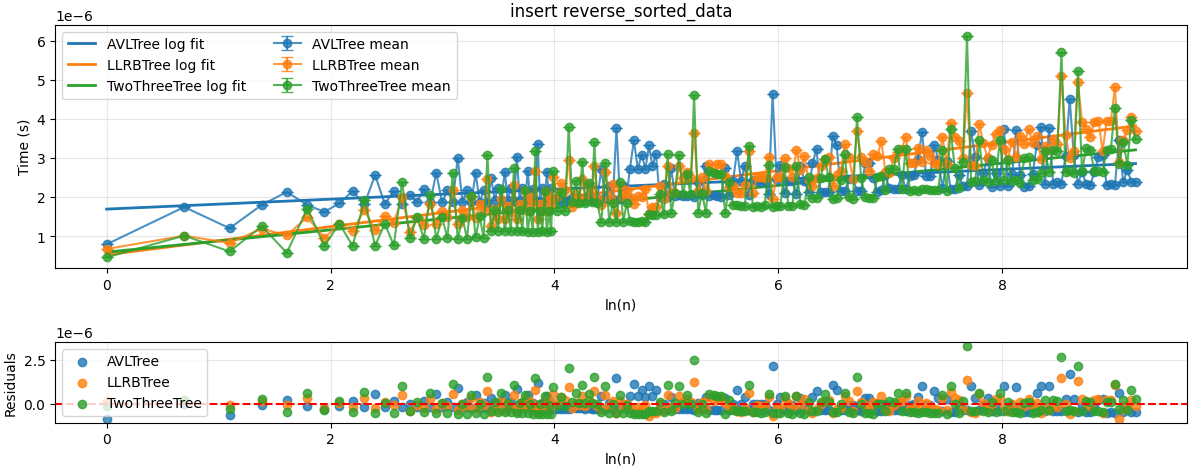
\includegraphics[width=0.6\textwidth]{3.png}
    \vspace{-1em}
    \caption{Comparison of insertion time under reverse-sorted keys.}
    \label{fig:4}
\end{figure}
\vspace{-2em}
\section{Comparative assessment}
Each data structure showed a strong logarithmic asymptotic growth. With random keys, the PMCC was greater than 0.99 for each plot, and the RMSEs were low (each < 5 nanoseconds)  evidence to the fact that tree searches and insertions are indeed an $O(logn)$ operation in the average case.

The searching plots for AVL and LLRB trees showed nearly identical profiles - they are both binary trees with the same search implementation, meaning comparisons at any node have the same cost. This implies the trees have a similar depth in the average case.

LLRB trees have at most a depth of about $2log_2n$  \cite{sedgewick}, and AVL trees roughly $1.44log_2n$ \cite{mount}.
AVL trees maintain a costly invariant to achieve this lower upper-bound on depth but the results show that the theoretical bound on height fails to improve real-world performance. It is likely that drawing keys from even distributions had a self-balancing effect, giving both trees a better-than-expected balance, and explaining their similarities.

Despite still growing logarithmically, searching 2-3 trees was slower than AVL and LLRB, taking roughly $~2.5$x the time in trees of size 10,000. This was a counter-intuitive result. 2-3 trees have a well-balanced structure. A search can take at most $2log_3N$ comparisons \cite{algorithms}, which is less than that of an AVL or LLRB tree. But these bounds are on the worst case: AVL and LLRB trees seemed to hold a better than worst-case balance. And the 2-3 tree’s rigid structure means it always shows near-to-worst-case performance. Moreover, the 2-3 tree’s search uses python list operations - which are notably slower than comparison-based operations used in the other trees. It is plausible that both factors contributed to the performance gap.

Successful searches seemed to take the same amount of time as (or just less than) failed searches in every tree. In a balanced tree, most keys lie close to the leaves – half of the nodes in a balanced binary tree are leaf nodes, so this was not unexpected. 

For insertions, AVL trees were comparably slower than 2-3 and LLRB trees, taking about $2$x the time than LLRB and 2-3 trees for trees of size 10,000. Most of the cost of an insertion comes from the fix-up operation. AVL’s re-balancing has five cases; LLRB's has three. AVL recalculates heights at every node on every insertion, whereas LLRB and 2-3 trees' chaining operations often terminate quickly. This highlights the main trade-off of using AVL trees: while improving search times in theory, the invariant is expensive to maintain.

With random inputs, 2-3 trees just outperformed LLRB trees.  But this pattern broke down with the edge cases: on sorted input, LLRB trees were faster than 2-3 trees, and with reverse sorted input, the opposite was true.  While 2-3 and LLRB trees showed lots of variation when tested on edge cases, AVL trees were in general, much more stable on all inputs.

Across all trees, the data showed few outliers. $3.3$ per-cent of  insertions, and $4.0$ per-cent of searches were recorded as such in randomly constructed trees. Outliers were always positive ($> Q_3 + 5*IQR$). These spikes were caused by OS scheduling changes, or garbage collection. 

The results show different data structures are suited to different tasks. On randomly sampled input, 2-3 trees were the best for insertions, but LLRB and AVL were better for searches. LLRB trees outperformed or matched AVL trees on all tests, making them seem like a better choice, but AVL trees showed much more stability in insertion times, and were less susceptible to edge-case breakdowns than both LLRB and 2-3 trees. For insertion-heavy workloads, 2-3 trees are the better option, for search-heavy workloads, LLRB trees are the best choice, unless edge-case stability matters, in which case AVL trees might be better suited to the task.
\vspace{-1em}
\section{Team contributions}
\begin{tabular}{|l|l|l|l|}
\hline
Harry Mannix&  25005445&  2-3, section 3 and stats& ($33.33\%$)\\\hline
          Ben Dalton&            25012352&         AVL, section 1, testing&          ($33.33\%$)\\
%% more entries as needed
\hline
 Yuheng Zhu& 25105536& LLRB, section 2, graphs&($33.33\%$)\\\hline
\end{tabular}
\vspace{-1em}
\printbibliography
\end{document}
